% LaTeX style file for Ph.D. thesis document
% Institution: Kyungpook National University (KNU)
% 
% (c) Gwenaelle Cunha Sergio (gwena.cs@gmail.com)
% and
% (c) Dennis Singh Moirangthem (mdennissingh@gmail.com)
%
% Please note:
%    1. Compile with XeLatex
%    2. This was not made for monetary purposes and it is free for anyone to use. However, if you do use it or modify it, please acknowledge this work by mentioning this original source code.
%

% !TeX program = lualatex

\documentclass[12pt]{report}

\usepackage{thesis}
%%%%%%%%%%%%%%%%%%%%%
% Required packages %
%%%%%%%%%%%%%%%%%%%%%

% Document formatting
\usepackage{adjustbox}
\usepackage{ragged2e}
\usepackage{setspace}
\usepackage{times}
\usepackage{latexsym}
\usepackage{url}
\usepackage{etoolbox}
\usepackage{graphicx}
\usepackage{url}
\usepackage{amsmath}
\numberwithin{equation}{chapter}
\usepackage{amssymb}
%\usepackage{subfigure}
\usepackage{color}
\usepackage{multirow}
\usepackage{comment}
\usepackage{pdflscape}
\usepackage{bibentry}
\usepackage{caption}
\usepackage{booktabs}
\usepackage[noadjust]{cite}
\usepackage{fancyhdr}


% Needed for \phantomsection definition
\usepackage{hyperref}

% Images
\usepackage{graphicx}
\usepackage{subfig}

% Indents first paragraph
\usepackage{indentfirst}

\usepackage{titlesec}

\usepackage[]{algorithm2e}

\titleformat{\chapter}[display]
{\normalfont\bfseries}{}{0pt}{\Huge}
\setlength\parindent{0pt}

\newtheorem{defn}{Definition}

% Suppress badness warnings
\hbadness=99999

\DeclareMathOperator*{\argmax}{arg\,max}
\DeclareMathOperator*{\argmin}{arg\,min}
\DeclareMathOperator*{\softmax}{softmax}
\DeclareMathOperator*{\aggr}{\boxplus}
\newcommand{\norm}[1]{\left\lVert#1\right\rVert}


%%%%%%%%%%%%%%%%%%%%%%%%
% Document starts here %
%%%%%%%%%%%%%%%%%%%%%%%%
\begin{document}
\onehalfspacing
\makecover
\makeinnercover\newpage
\pagenumbering{arabic}
%\thispagestyle{empty}
\addtocounter{page}{1}
\tableofcontents \newpage
\listoffigures \newpage

\setstretch{1.0}
\phantomsection~\label{sec:ref}
\addcontentsline{toc}{section}{Summary of Notation} \pagebreak

%%%%%%%%%%%%%%%%%%%%
% Rest of document %
%%%%%%%%%%%%%%%%%%%%
\setcounter{figure}{0}
\setcounter{table}{0}
\section{Introduction}~\label{sec:introduction}
This is the template
 \pagebreak

\setcounter{figure}{0}
\setcounter{table}{0}
\chapter{Preliminaries}~\label{sec:preliminaries}

\section{Image segmentation}~\label{sec:prel_imagesegmentation}

Image segmentation or image partitioning is defined as the process of dividing a digital image into sets of pixels known as the objects in the image.\\
There are many variations concerning the segmentation method itself as well as the goal that is to be achieved. With the rise of CNNs, nowadays these methods are usually fully or by parts learning based. That means, that some parameterized function is optimized in order to approximate some target which can only be described by prior knowledge and/or by drawing samples from a target distribution. For the task of image segmentation these samples are of the form $(x, y)$ which is a realization of a random variable $(X, Y)$ with probability distribution $P_{X, Y}(x, y)$. Samples represent the raw input image $x$ that is to be segmented and the desired segmentation $y$ also referred to as label or label image. The goal is to learn a function $f(x)$ such that it approximates $\mathbb{E}[Y|X=x]$ at best. Since $P_{X, Y}$ is initially not known and only few samples and/or some prior knowledge on its properties are available, the approximation can only be achieved by the Monte Carlo estimate of the expectation obtained from those samples and by dexterous use of the prior knowledge. \\
Some of the variations of learning based methods for image segmentation are distinguished by their level of supervision during the optimization. This is mainly defined by the amount of data samples and prior knowledge on the distribution $P_{X, Y}$ that is available and used by the method.

\begin{itemize}
	\item \textbf{supervised segmentation} is the highest level of supervision. Here only samples from $P_{X, Y}$ are available to the method. If enough samples are available such that all regions in the domain of the distribution are covered sufficiently, this is usually all one needs to arrive at a satisfactory result. However for most applications the set of available samples is very limited.
	\item \textbf{unsupervised segmentation} is the lowest level of supervision. Here no samples from $P_{X, Y}$ are available to the method. The optimization method has to completely rely on prior knowledge on the underlying distribution. Realizations of $X$ are usually still available and can be used for the learning process.
	\item \textbf{semi-supervised segmentation} is the transition between the previous two. Similar to supervised learning, semi-supervised learning uses samples from $P_{X, Y}$, but not only. There are also realizations of $X$ available as well as some prior knowledge on $P_{X, Y}$ which is used for the learning process.
	\item \textbf{self-supervised learning} is usually referred to when the method generates some kind of supervisory signal for itself. E.g. an automated labeling procedure to generate sample approximations $(x, \bar{y})$. Self-supervised learning is a special case of unsupervised learning.
\end{itemize}

Other variations that focus more on the goal that should be achieved are

\begin{itemize}
	\item \textbf{semantic segmentation} is the process of assigning class labels to each pixel in the image. Different objects instances of the same class are labeled equally. Usually only some object classes of interest get a unique class label assigned to. All other object classes receive the label background.
	\item \textbf{instance segmentation} is similar to semantic segmentation in the sense that each pixel in the image is assigned a label to. This label attributes a pixel either to background or to an instance of an object class. Therefore different objects of the same class are labeled differently. Here the label of an instance is also referred to as object id.
	\item \textbf{panoptic segmentation} is a fusion of the previous two. For all pixels belonging to instances of some defined set of classes, instance segmentation is performed. For the remaining pixels, semantic segmentation without a background label is performed. The object instances for which instance segmentation is performed are referred to as "things" (objects with a well defined shape like cars, buildings ...) and the object instances for which semantic segmentation is performed are referred to as "stuff" (background regions like grass, sky ...).
\end{itemize}
\section{Reinforcement Learning (RL)}~\label{ssec:rl}
Please note that this is an aggressively shortened summary. For a deeper introduction please refer to \cite{SB_all}.
The Reinforcement Learning problem originates from the idea of learning by interacting with an environment. The object that is learning is doing so by retrieving information from cause and effect. The causal model that is learned in such a way is updated with each change of the environment that can be related to some action. Therefore, the learned model fits the true model increasingly better with the number of induced causes and observed effects.\\
This type of learning problem can be modeled by "Finite Markov Decision Processes". Such processes usually need the following elements:\\

\begin{itemize}
	\item \textbf{Environment} The environment is a dynamic model of some complex process.
	\item \textbf{State} The state $s_t$ is generated by the environment. It changes over time according to the dynamics within the environment.
	\item \textbf{Action} An action $a_t$ is a cause that might change the state of the environment. Actions are produced by the agent.
	\item \textbf{Reward} The reward $r_t$ is a scalar value that is produced by the environment and received by the agent.
	\item \textbf{Agent} The agent is a instance which generates actions and observes the caused change of the state of the environment.
	\item \textbf{Policy} A policy $\pi(a_t|s_t)$ is a probability distribution over the set of possible actions at a time step. A agent is essentially defined by its policy as each action that is taken is sampled from that policy.
\end{itemize}

The model with its signal flows is depicted in figure \ref{fig_rl_gen}

\begin{figure}
	\centering
	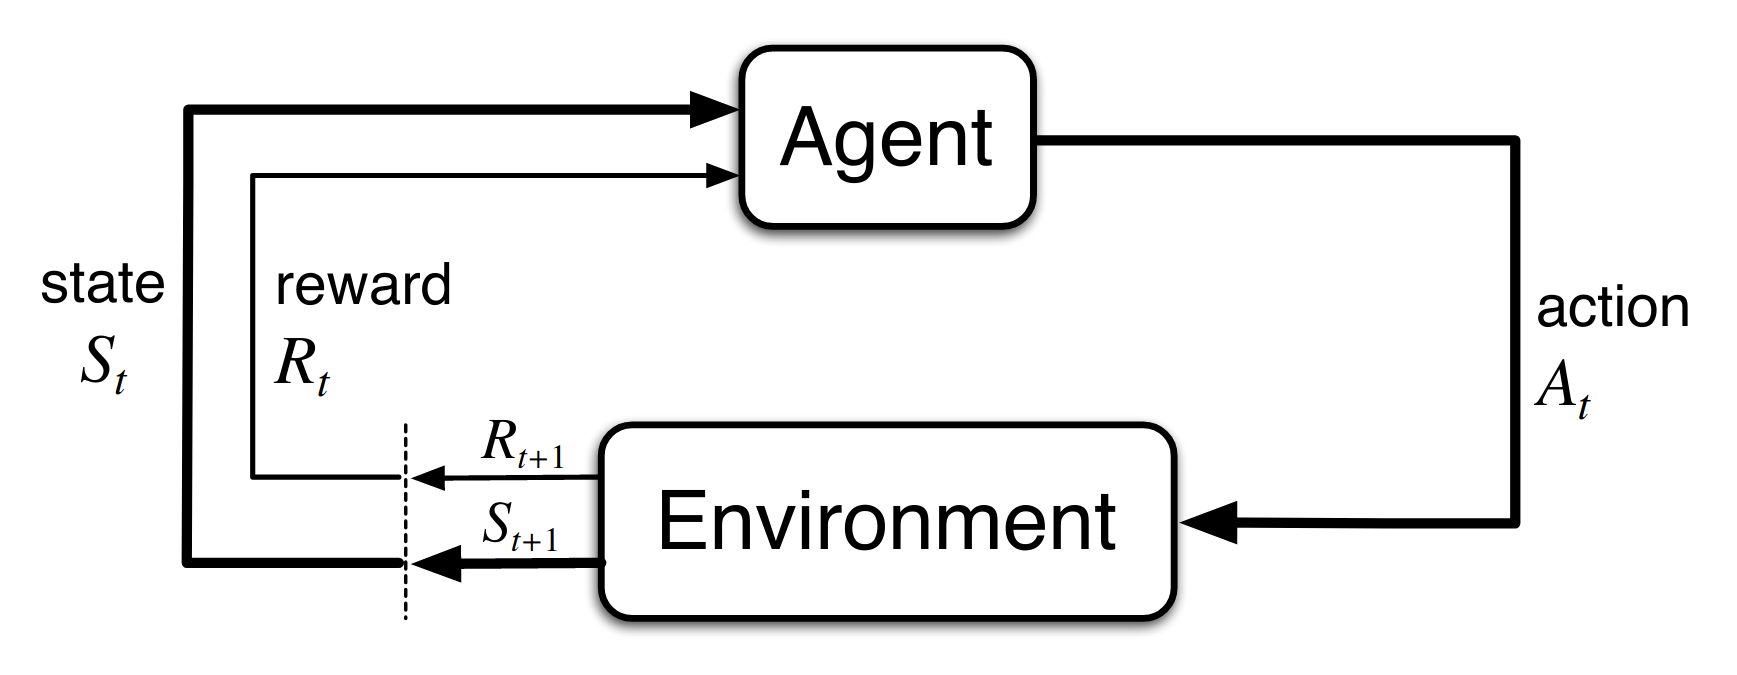
\includegraphics[width=0.8\textwidth]{figures/rl/agent_env_interface}
	\caption{agent environment interaction \cite{SB_all}}
	\label{fig_rl_gen}
\end{figure}

All signals in this model are time dependent. 
Such a model satisfies the Markov Property if next $s'$ and reward $r$ only depend on the current action-state tuple $(s, a)$. If assuming finite state and action spaces together with the Markov Property gives a Finite Markov Decision Process. The environment dynamics can therefore be represented by the bivariate probability distribution
\begin{align}
	p(s', r|s, a) = Pr\{r_{t+1}=r, s_{t+1} = s' | s_t=s, a_t=a\}
\end{align}
Further, if $a_t$ is sampled from $\pi(a_t|s_t)$ the Markov Property induces conditional independence of $(s_{t-1}, r_{t-1})$ and $(s_{t+1}, r_{t+1})$ given $s_t$. \\

The agents task is to predict a policy that maximizes the expected future rewards. This objective is given by
\begin{align}
	\argmax_{\pi}\mathop{\mathbb{E}}_{p_{\pi}}\left[\sum_{t=0}^T r_t | s_0\right]
\end{align}
Here T marks the time limit of the process and $p_{\pi}$ represents the environment dynamics following a action history sampled from $\pi$.\\

\subsection{Value functions}
Most methods of solving eq. (1.2) use so estimations of so called value functions. This are functions that provide a quality measure for an agent evaluating a state-action tuple. \\
Commonly three value functions are used. The state-value function, the action-value function and the advantage-value function. They all depend on the expected discounted future rewards
\begin{align}
	g_t = \sum^{T-t-1}_{k=0} \gamma^k r_{t+k+1} .
\end{align}
Here $\gamma$ is referred to as the discount factor. Its value usually determines how prospective future rewards are weighted in the value function. E.g if $\gamma<1$ rewards that are closer to $t$ get a higher weight than those that are occuring at a later time. For $\gamma>1$ the contrary holds.\\
The state-value function is defined by
\begin{align}
	V_{\pi}(s) = \mathop{\mathbb{E}}_{p_{\pi}}\left[g_t|s_t=s \right]\text{,}
\end{align}
the action-value by
\begin{align}
	Q_{\pi}(s, a) = \mathop{\mathbb{E}}_{p_{\pi}}\left[g_t|s_t=s, a_t=a \right]
\end{align}
and finally the advantage-value by
\begin{align}
	A_{\pi}(s, a) = Q_{\pi}(s, a) - V_{\pi}(s)
\end{align}
it follows
\begin{align}
	V_{\pi}(s) = \mathop{\mathbb{E}}_{a\sim\pi}\left[ Q_{\pi}(s, a)\right]
\end{align}

\noindent Usually the objective is to maximize either one or both of the value functions.
Note that, $\max_{\pi}V_{\pi}(s)$ and $\max_{\pi}Q_{\pi}(s, a)$ satisfy Bellman's principle of optimality. Hence they can be solved exactly by Dynamic Programming. This is referred to as the tabular solution. However for most problems this is not feasible and the value functions are approximated by neural networks. \\

\subsection{Q-learning}
Q-learning is a method to find the action-value maximizing policy by using temporal differences. This often the backbone of policy gradient algorithms. Let
\begin{align}
\pi(\cdot|s) = \softmax_{a}Q_{\pi}(s, a)
\end{align}
then the objective is to approximate $Q_{\pi}$ which is achieved by the temporal difference loss
\begin{align}
\mathcal{L}_{TD} = \frac{1}{2} \left(r_{t+1} + \gamma \max_{a}Q_{\pi}(s_{t+1}, a) - Q_{\pi}(s_t, a_t)\right)^2
\end{align}
this kind of approximation is usually referred to as one step TD method. The optimality follows directly and the convergence of the approximation under certain conditions has been proven in \cite{SBQL}.\\
In contrast to one step TD methods there are Monte Carlo methods which collect the loss over whole episodes where one episode is defined by the history of temporal differences between a starting state and an end state. This methods are often solved by eligibility traces \cite{SBeligibility}. \\
Optimizing eq (1.8) is referred to as on-policy policy optimization where the target policy $\pi$ is the policy which is used when actions are sampled. This however is problematic as the target policy is defined by eq (1.7) depending on $q_{\pi}$ which is not trustworthy as this is the function that is to be approximated. In order to have more control over the sampling of actions which is usually referred to as exploration a data collection policy $\mu(a|s)$ is used. Therefore in an off-policy setting eq (1.8) becomes
\begin{align}
\mathcal{L}_{TD} = \frac{1}{2} \left(r_{t+1} + \gamma \max_{a}Q_{\mu}(s_{t+1}, a) - Q_{\mu}(s_t, a_t)\right)^2\text{.}
\end{align}
and during inference 
\begin{align}
\bar{\pi}(\cdot|s) = \softmax_{a}Q_{\mu}(s, a)
\end{align}
is used. There are many solutions to overcome the distribution mismatch between $\pi$ and $\mu$. Many use importance sampling or variance reduction techniques.\cite{liu2018breaking}

\subsection{Policy gradient methods}

This class of methods optimizes the parameters $\theta$ that define the statistics of a policy $\pi_\theta(a|s)$. Let 
\begin{align}
\rho(\pi) = \sum_{t=1}^{\infty}\mathop{\mathbb{E}}_{\substack{s\sim d_\pi(s) \\ a\sim \pi(a|s)}} \left[ r_t|s_0 \right]
\end{align}
be the expected, discounted future reward per step and let
\begin{align}
d_\pi(s) = \sum_{t=0}^\infty \gamma^t Pr\left\{s_t=s|s_0, \pi\right\}
\end{align}
be the discounted stationary distribution of states under $\pi$. Then
\begin{align}
\frac{\partial\rho_\pi}{\partial\theta} = \sum_s d_\pi(s)\sum_a \frac{\partial\pi(a|s)}{\partial\theta} \bar{Q}_\pi(s,a)
\end{align}
Is the policy gradient with which gradient ascent on the policy can be performed in order to maximize $\rho$. A proof and a thorough discussion can be found in \cite{PGBS}. Note that the policy gradient is on-policy and that $\bar{Q}_\pi$ is an approximation of $Q_\pi$.\\
Since $\pi$ is a probability distribution it follows $\sum_a\frac{\partial\pi(a|s)}{\partial\theta}=0, \forall s \in S$. Therefore
\begin{align}
\frac{\partial\rho_\pi}{\partial\theta} = \sum_s d_\pi(s)\sum_a \frac{\partial\pi(a|s)}{\partial\theta}\left[ \bar{Q}_\pi(s,a)+b(s)\right],\text{\hspace{12mm}} b:S\rightarrow \mathop{\mathbb{R}}
\end{align}
the function $b$ is called a baseline and is often used to reduce variance and bias of the gradient ascent update step. Using $\frac{\nabla_\theta\pi(a|s)}{\pi(a|s)} = \nabla_\theta ln(\pi(a|s))$ and $\mathop{\mathbb{E}}_{x\sim p(x)}[f(x)] = \sum_{x}p(x)f(x)$, rewriting eq (1.13) yields
\begin{align}
\frac{\partial\rho_\pi}{\partial\theta} = \mathop{\mathbb{E}}_{\substack{s\sim d_\pi(s) \\ a\sim \pi(a|s)}}\left[ \nabla_\theta ln (\pi(a|s))\left[ \bar{Q}_\pi(s,a)+b(s)\right]\right]
\end{align}
In practice where there are large state and action spaces the expectations w.r.t $s$ and $a$ become infeasible to obtain. Using $\mathop{\mathbb{E}}_{x\sim p(x)}[f(x)] = \frac{1}{n}\sum_{n}f(x), n\rightarrow\infty, x\sim p(x)$ , ample based learning uses enough samples of $s$ and $a$ in order to obtain a good enough approximation of the expectations. Therefore eq. (1.15) becomes

\begin{align}
\frac{\partial\rho_\pi}{\partial\theta} = \frac{1}{n}\sum_{n} \nabla_\theta ln (\pi(a|s))\left( \bar{Q}_\pi(s,a)+b(s)\right),\text{\hspace{8mm}} s\sim d_\pi(s), \text{\hspace{4mm}} a\sim \pi(a|s), \text{\hspace{4mm}} n\rightarrow\infty
\end{align}

This leads to Actor Critic methods (A2C) where there are two instances that are updated in a turn based fashion. The critic is the value-function approximation and the actor is approximating the policy. Intuitively the critic evaluates the action taken by the actor who uses this evaluation to scale its gradient update (this is the role of $\bar{q}_\pi$ in eq (1.13)).

\subsection{Maximum Entropy Reinforcement Learning}
In off-policy settings it is common to use a data collection policy $\mu$ which has a large entropy in order to encourage exploration of the action and state spaces. The principle of maximum causal entropy has been introduced by \cite{AAAIziebert} and has been elaborated on among others by \cite{DBLP:journals/corr/HaarnojaTAL17}. The key idea is to incorporate an entropy term into the objective function acting like a regularizer. 

\begin{align}
\rho^{\mathcal{H}}(\pi) = \sum_{t=1}^{\infty}\mathop{\mathbb{E}}_{\substack{s_t \sim d_\pi(s_t) \\ a_t \sim \pi(a_t|s_t)}} \left[ r_t + \alpha(t) \mathcal{H}(\pi(\cdot | s_t))|s_0 \right]
\end{align}
Here $\alpha$ is a non-negative regularization weight which is usually monotonically decreasing with increasing $t$ and $\mathcal{H}$ is some entropy measure. If $\alpha$ becomes $0$ eq. (1.17) becomes equal to eq. (1.11), therefore, intuitively $\alpha$ should be high in the early phase of training the policy and the value function and converge to $0$ as the policy gets closer to the perfect policy and therefore can afford to have more certainty in its prediction.
This objective is on-policy and still gives control over the exploration behavior. Usually it does not bother if the policy has high entropy, since during inference the action where "\pi" has maximum probability is selected. This makes especially unimodal distributions attractive. They fixate on single actions and they imply few parameters only that need to be learned (e.g. mean and variance of normal distributions). However often more expressive multimodal distributions fit the true distribution which is approximated better. 
In \cite{DBLP:journals/corr/abs-1906-02771} this idea has been extended by using  normalizing flows. Normalizing flows \cite{papamakarios2019normalizing} are based on the idea of transforming a probability density function by letting each sample undergo a transformation. If this transformation is a diffeomorphism the probability of the transformed sample can be determined. Let $T$ be a diffeomorphism of a real vector $u$ sampled from $p_u(u)$.

\begin{align}
	x=T(u) \text{\hspace{5mm}where\hspace{5mm}} u\sim p_u(u)
\end{align}
then
\begin{align}
p_x(x)=p_u(T^{-1}(u)) |detJ_T(u)|^{-1}
\end{align}
where $J_T(u)$ is the Jacobian matrix of $T$ w.r.t. $u$. I practice an invertible neural network can be trained to transform a simplistic density function into a more expressive one.\\
E.g. let the agent predict mean and variance of a Normal distribution. Actions are the in the data collection process sampled from a transformed Normal distribution where the transform encourages entropy and maybe also multiple modes. Assuming the sampling happened using reparametrization the log probabilities and their gradient in eq (1.14) can still be calculated. This is a on-policy training with a expressive density function and the advantage is that easy reparameterization tricks can still be used since the sampling itself is happening from the base distribution.

\subsection{Soft Actor-Critic (SAC)}
This algorithm was introduced by \cite{haarnoja2018soft}. They aim to maximize the objective in eq. (1.17). Particularly they focus on the selection of the weight factor $\alpha$ and show, that it can be seen as a learnable parameter which is trained jointly with actor and critic networks.\\
SAC is derived from the soft policy iteration where the temporal difference equation for the action value depends on the soft value function which is
\begin{align}
	V_{\pi}(s_t) = \mathop{\mathbb{E}}_{a \sim \pi(a|s_t)} \left[ Q_{\pi}(s_t, a) - \alpha log( \pi(a|s_t)) \right]
\end{align}
the negative log probabilities are the entropy measure in eq. (1.18). The action value function loss yields
\begin{align}
	\mathcal{L}_{critic} = \frac{1}{2}(Q_{\pi}(s_t, a_t) - (\gamma \mathop{\mathbb{E}}_{s_{t+1} \sim d_{\pi}(s)} \left[ V_{\pi}(s_{t+1})\right] + r_t)) ^ 2
\end{align}

For the policy improvement step the policy is updated such that it approximates $\softmax_a(\frac{1}{\alpha}Q_{\pi}(s, a))$ where $Q_{\pi}$ is the soft action value function, learned by minimizing eq (1.21). The loss for the policy then yields

\begin{align}
\mathcal{L}_{actor} = DKL_{a}\left[ \pi(a| s_t) \bigg|\bigg| \frac{exp(\frac{1}{\alpha} Q_{\pi}(s_t, a))}{Z(s_t)} \right]
\end{align}

here, $DKL_{a}$ is the Kullback Leibler Divergence over the actions. $Z(s_t)$ is the partition function of the distribution. 

\begin{align}
	Z(s_t) = \sum_a Q_{\pi} (s_t, a)
\end{align}

It is usually too expensive to evaluate $Z(s_t)$ since it involves integrating/summing over the action value space which means many forward passes through the neural network that represents $Q_{\pi}$. Since $\mathcal{L}_{actor}$ is minimized by gradient descent methods only the gradient is needed. If one expands the KL-divergence term, $Z(s_t)$ becomes additive and therefore vanishes once the gradient is obtained.\\
Note that $\alpha$ gives control over the differences between action values and therefore over the entropy of the resulting distributution. \emph{lemma 2} in \cite{haarnoja2018soft} claims the improvement of $Q_{\pi}$ with each optimization step of $\mathcal{L}_{actor}$.\\
The gradient of eq. (1.23) w.r.t. the parameters $\theta$ of $\pi$ yields

\begin{align}
\nabla_\theta \mathcal{L}_{actor} = \nabla_\theta \mathop{\mathbb{E}}_{\substack{s_t \sim d_\pi(s_t) \\ a_t \sim \pi(a_t|s_t)}} \left[ \alpha log(\pi(a_t|s_t)) - Q_\pi(s_t, a_t) \right]
\end{align}

approximating eq. (1.24) by a sample based method yields

\begin{align}
\nabla_\theta \bar{\mathcal{L}}_{actor} = \nabla_\theta \left[ \alpha log(\pi(a_t|s_t)) - Q_\pi(s_t, a_t) \right]
\end{align}

minimizing this loss by a gradient descent method involves backpropping through a sampling procedure. This can be made differentiable by the reparameterization trick \cite{kingma2013autoencoding}.

\cite{haarnoja2018soft} also provides a method to determine the entropy adjustment $\alpha$ such that it takes the minimal value needed to maximize the maximum entropy objective eq. (1.17) assuming a fixed policy $\pi$.

In practice, reinforcement learning problems have high dimensional action spaces but only one dimensional rewards. Therefore the learned action value function of the critic is also one dimensional in contrast to the actor who predicts the statistics of the policiy for each action dimension. Then the joint probability is the product of probabilities over all actions. This results in summing the log probabilities in eq. (1.25)

\subsection{Common optimization methods}
There are numerous optimization methods for reinforcement learning problems. This is just a listing of only very few but important ones, reviewed and tested in \cite{hessel2017rainbow}.

\begin{itemize}
	\item \textbf{Double Q-learning} \cite{DBLP:journals/corr/HasseltGS15} Conventional Q-learning is affected by an overestimation bias of action values. Decoupling the action selection from its evaluation by learning two action value networks independently resulting in the loss
	
	\begin{align}
		\mathcal{L}_{TD} = \frac{1}{2} \left(r_{t+1} + \gamma Q_{\pi}^{(\bar{\phi})} \left( s_{t+1}, \argmax_{a}Q_{\pi}^{(\phi)}(s_{t+1}, a) \right) - Q_{\pi}^{(\phi)}(s_t, a_t)\right)^2\text{.}
	\end{align}
	Here $\phi$ and $\bar{\phi}$ are the parameters of the independently trained action value functions respectively. A similar method trains two action value functions independently and and takes for all evaluations the min value of the two network predictions. Both methods show a reduction in overestimation as shown in \cite{DBLP:journals/corr/HasseltGS15}.
	
	\item \textbf{Prioritized replay} During data collection, the tuples $(s_t, a_t, r_{t+1}, s_{t+1})$ are stored in a replay buffer and during training phases then sampled uniformly from the buffer. In \cite{schaul2015prioritized} the sampling is not uniform but rather with a probability $p_t$ relative to the last encountered loss of that replay tuple.
	\begin{align}
		p_t \propto \mathcal{L}_{TD} ^ \omega \text{.}
	\end{align}
	Raising the loss to the power of the parameter $\omega$ determines the shape of the distribution. New transitions that did not produce a loss yet are always sampled with maximum priority.
	
	\item \textbf{Multi-step learning} Q-learning bootstraps from single step temporal difference losses. \cite{SBQL} introduced multi-step temporal differences which is the transition from Monte Carlo methods to single step temporal difference methods. The $n$-step return is defined as 
	
	\begin{align}
		r_t^{(n)} \equiv \sum_{k=0}^{n-1} \gamma_t^{k} r_{t+k+1}
	\end{align}
	
	then the multi step TD loss yields,
	
	\begin{align}
		\mathcal{L}_{TD} = \frac{1}{2} \left(r_{t+1}^{(n)} + \gamma^{n} \max_{a}Q_{\pi}(s_{t+n}, a) - Q_{\pi}(s_t, a_t)\right)^2
	\end{align}
	
	optimizing multistep TD losses with $n$ sampled uniformly from the interval $[1..T]$ results in faster learning as shown in \cite{SBQL}.
	
	\item \textbf{Dueling networks} This is an optimization method based on the neural network atrchitecture of value functions in value based RL and was introduced by \cite{DBLP:journals/corr/WangFL15}. It features one state-value and one advantage-value stream of computation that both share a common state feature extractor network $f(s)$. This leads to this factorization of action-values
	\begin{align}
		Q_{\pi}^{(\phi)}(s, a) = V_{\pi}^{(\eta)}(f^{(\xi)}(s)) + A_{\pi}^{(\psi)}(f^{(\xi)}(s), a) - \frac{\sum_{a'} A_{\pi}^{(\psi)}(f^{(\xi)}(s), a')}{N_{actions}}
	\end{align}
	
	Here $\eta, \psi$ and $\xi$ are the parameters of the state-value function, the advantage-value function and the state feature extractor respectively. $\phi$ is the concatenation of $\eta, \psi$ and $\xi$.\\
	The last term in eq. (1.31) approximates $\mathop{\mathbb{E}}_{a' \sim \pi} A_{\pi}^{(\psi)}(f^{(\xi)}(s), a')=0$, this equality follows from combining eq (1.6) and eq(1.7). Then eq. (1.31) follows from eq (1.4), eq (1.5) and eq (1.6).\\
	This method outperforms vanilla, value based RL methods on common RL benchmarks. 
	
\end{itemize}


\section{Geometric deep learning}~\label{sec:gcn}
\noindent Convolutional neural networks use the convolution operation to "filter" a regular grid graph of certain dimension with a filter consisting of learnable parameters. Graph convolution, as introduced by \cite{bruna2013spectral} generalizes this notion of convolutional filtering to arbitrary graphs. Through that it is possible to learn functions on non eucledian, structured domains that have a notion of locality.\\
Since then the field developed rapidly, \cite{Bronstein_2017} provides a good overview of the research that was done so far.\\
Most of the research focuses on the application where graphs are constructed from discretizations of 2-dimensional manifolds, embedded in a 3-dimensional eucledian space, usually called point clouds. However the principle can be used for arbitrary graphs that contain features in their nodes.\\
Typically there are two equivalent definitions of convolution on graphs. One is the spectral definition which suffers from large complexity in terms of memory and time. The other one is a spatial construction motivated from signal flows on graphs which is much faster as it operates with sparse representations of the graph. A quick summary of the latter as in \cite{gilmer2017neural} is given below. \\

Let a graph be represented by $G=(X, (A, E))$ where $X\in \mathbb{R}^{N\times m}$ is a node feature matrix of $N$, $m$-dimensional node feature vectors, with nodes ecoded as $i \in[1..N]$. $A$ is a set of adjacency tuples where $A\in \mathbb{N}^{2\times |E|}$ encodes the set of $|E|$ edges with $n$-dimensional edge features $E \in \mathbb{R}^{|E|\times n}$.

The generalization of the convolutional operator, locally expressed by means of the neighborhood $\mathcal{N}(i)$ around node $i$, is

\begin{align}
	\vec{x}_i^\prime = \gamma \left(\vec{x}_i, \aggr_{j \in \mathcal{N}(i)}  \phi \left(\vec{x}_i, \vec{x}_i, \vec{e}_{ij} \right) \right)
\end{align}

where $\aggr$ is a differentiable and permutation invariant function such as the sum or the mean. $\gamma$ and $\phi$ are differentiable functions represented by multi layer perceptrons. This convolution is also referred to as message passing scheme. All this convolution operations w.r.t. to each node in the graph allow parallel computation what makes this schemes fast.




\section{Mutex watershed}~\label{sec:mtx_wtsd}
The Mutex Watershed algortihm introduced in \cite{wolf2019mutex} is a image partitioning algorithm based on watersheding that is able to operate without a prior seeding.\\
Like most image partitioning algorithms it is defined on a graph $G=(V, E^+ \cup E^-, W^+ \cup W^-)$ with a set of vertices $V$, a set of edges as the disjoint union of attractive edges $E^+$ and repulsive edges $E^-$ and a set of corresponding edge weights $ W^+ \cup W^-$. Each vertex in this graph represents uniquely a pixel in the corresponding image. The edge weights are based on the affinity between the incidental vertices of the respective edge. The affinity between two nodes $i$ and $j$ is the probability $p_{ij}$ of the nodes belonging to the same partition in the posterior partitioning. These affinities can be based on differences in pixel intesities or be predicted by e.g. a CNN. \\
Attractive edges $e_{ij}^+ \in E$ have edge weights $w_{ij}^+ \in W$ with $w_{ij}^+ = p_{ij}$. Repulsive edges $e_{ij}^- \in E$ have edge weights $w_{ij}^- \in W$ with $w_{ij}^- = 1-p_{ij}$. \\
A partitioning on $G$ is defined by the disjoint union of a set of attracive and a set of repulsive edges by the active set $A=A^+ \cup A^-$ that encode hard merges and mutual exclusions of vertices.\\
To represent a valid partitioning, the set $A$ has to satisfy cycle constraints. Defining the set $\mathcal{C}_i(A)$  with $A\subseteq E$ as the set of all cycles in $A$ with exactly $i$ active repulsive edges
\begin{align}
	\mathcal{C}_i(A) := \left\{ c \in cycles(G) \vert c \subseteq A \text{  and  } |c \cap E^- | = i \right\},
\end{align}
a valid partitioning can only be inferred from an active set $A$ if $\mathcal{C}_1(A) = \emptyset $. If additionally $\mathcal{C}_0(A) = \emptyset $, the algorithm can be defined as the search for the minimal spanning tree in each partition.\\
\vspace{8mm}\\
\begin{algorithm}[H]
	\KwData{weighted graph $G=(V, E^+ \cup E^-, W^+ \cup W^-)$}
	\KwResult{clusters defined by spanning forest $A^\star \cap E^+$}
	Initialization: $A = \emptyset$\;
	\For{$(i, j) = e \in(E^+ \cup E^-)$ in descending order of $W^+ \cup W^-$}{
		\If{$\mathcal{C}_0(A \cup \{ e \}) = \emptyset$ and  $\mathcal{C}_1(A \cup \{ e \}) = \emptyset$}{
			$A \leftarrow A \cup e$ \;
		}
	}
	$A^\star \leftarrow A$ \;
	\Return $A^\star$
	\caption{Mutex Watershed \cite{wolf2019mutex}}
	\label{algo:mtx_wtsd}
\end{algorithm}
\vspace{8mm}

An example walk through of the algorithm is depicted in figure \ref{fig_mtxwtsd1}. \\

\begin{figure}
	\centering
	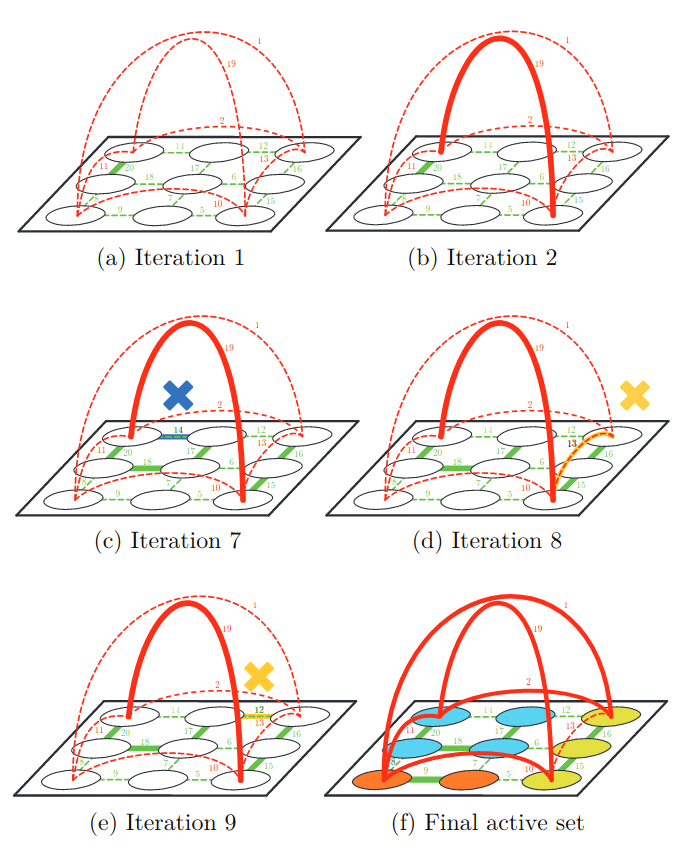
\includegraphics[width=0.5\textwidth]{figures/mutexwatershed/walkthrough}
	\caption{\cite{wolf2019mutex} Some iterations of algorithm \ref{algo:mtx_wtsd} applied to a graph with weighted attractive edges (green) and repulsive (red) edges. Edges that are part of the active set $A$ at each iteration are shown in bold. On termination (f), the connected components in $A \cap E^+$ represent the partitions of the final partitioning. Edges that are not added to $A$ because of the violation of $\mathcal{C}_0$ or $\mathcal{C}_1$ are highlighted in blue and yellow respectively.}
	\label{fig_mtxwtsd1}
\end{figure}

\newpage
Algorithm \ref{algo:mtx_wtsd} minimizes an energy functional that is defined by the active set $A$. This requires the following definition:
\begin{defn}
	\textbf{Dominant power} \cite{wolf2019mutex}: \\
	Let $G = (V, E, W)$ be an edge weighted graph, with unique edge weights $w_e \in \mathbb{R}_0^+$, $\forall e \in E$. Then $p \in \mathbb{R}^+$ is called a dominant power if:\\
	\begin{align}
		w_e^p > \sum_{\substack{t \in E \\ w_t < w_e}} w_t^p \text{\hspace{8mm},} \forall e \in E
	\end{align}
\end{defn}
 This allows the definition of the objective that is solved by algorithm \ref{algo:mtx_wtsd}
 
 \begin{defn}
 	\textbf{Mutex Watershed Objective} \cite{wolf2019mutex}: \\
 	Let $G = (V, E, W)$ be an edge weighted graph, with unique edge weights $w_e \in \mathbb{R}_0^+$, $\forall e \in E$ and $p \in \mathbb{R}^+$ a dominant power. Then the Mutex Watershed Objective is devined as the integer linear program:\\
 	\begin{align}
 		\min_{a\in {0,1}^{|E|}} - \sum_{e \in E} a_e w_e^p \\
		\text{s.t. \hspace{2mm}} \mathcal{C}_0(A) = \mathcal{C}_1(A) = \emptyset \text{, }\\
		\text{with \hspace{2mm}} A := \{ e \in E|a_e = 1 \}
 	\end{align}
 \end{defn}

\section{Image partitioning by multicuts}~\label{sec:multicut}
The multicut problem is a graph cuts problem that is in \cite{10.1007/978-3-642-23094-3_3} redefined for the image partitioning task. The unsupervised partitioning on a grid graph $G=(V, E)$ where each node $v \in V$ corresponds to a pixel in an image can be defined as the following minimization problem

\begin{align}
	\min_{x \in L^{|V|}} \sum_{uv \in E} \beta_{uv} I(x_u \neq x_v) \text{, \hspace{5mm}} L=\{ 1, ..., |V| \}
\end{align}

where $I$ is a indicator function that maps a boolean expression to $1$ if it is true and to $0$ otherwise. $L$ is the set of all possible labels, $\beta_{uv}$ is the edge cost that is active if $u$ has a different label than $v$. $x=(x_v)_{v\in V} \in L^{|V|}$ is a node labeling that defines a partitioning of $V$ into subsets of nodes $S_l$ assigned to class $l$ such that $\bigcup_{l \in L} S_l = V$. Eq. (2.38) defines the unsupervised partitioning problem where the maximum number of classes in the final labeling is the number of nodes $|V|$ in the graph $G$. Therefore the coefficients $\beta$ can depend on the data but are assumed not to depend on prior information about a fixed number of classes $L$. \\
A \emph{multicut} on a graph $G=(V,E)$ with a partitioning $\bigcup_{l \in L} S_l = V$ is defined as 
\begin{align}
	\delta(S_1, ..., S_k) := \left\{ uv \in E | \exists i \neq j : u \in S_i \text{\hspace{1mm}and\hspace{1mm}} v \in S_j \right\}
\end{align}
Where the sets $S_1, ..., S_k$ are called the \emph{shores} of the multicut.
To obtain a polyhedral representation of the set of multicuts on a graph on needs to define incidence vectors $\mathcal{X}(F) \in \mathbb{R}^{|E|}$ for each subset $F \subseteq E$:
\begin{align}
	\mathcal{X}_e(F) = \begin{cases}
	1, \text{\hspace{1mm}if\hspace{1mm}} e \in F \\
	0, \text{\hspace{1mm}if\hspace{1mm}} e \in E \backslash F
	\end{cases}
\end{align}
then the multicut polytope is given by
\begin{align}
	MC(G) := conv\left\{ \mathcal{X}(\delta (S_1, ..., S_k)) | \delta (S_1, ..., S_k) \text{ is a multicut of } G \right\}
\end{align}
and the unsupervised image partitioning problem eq. (2.38) can be written as the equivalent multicut problem

\begin{align}
	\min_{y \in MC(G)} \sum_{uv \in E} \beta_{uv} y_{uv}
\end{align}

defining cycle constraints allows to rewrite eq. (2.42) as the integer linear program (ILP)

\begin{align}
	\min_{y \in [0, 1]^{|E|}} & \sum_{uv \in E} \beta_{uv} y_{uv} \\
	 \text{s.t. \hspace{4mm}} \sum_{uv \in C} y_{uv} & \neq 1 \text{, \hspace{8mm}} \forall \text{ cycles } C \subseteq E 
\end{align}

The cycle constraints in eq. (2.47) enforce that $y$ lies inside the multicut polytope by guaranteeing that there are no active edges inside a shore. There are many solution methods for this problem. The one used in \cite{10.1007/978-3-642-23094-3_3} is based on iteratively solving the ILP in eq. (2.43) without cycle constraints initially, then finding violated constraints in the sense of eq. (2.44), adding them to the ILP and reiterate until there are no more violated cycle constraints.\\
Violated constraints can be found by projecting a obtained solution $y$ to the multicut polytope and checking for differences in the solution and the projection $y'$.
The projection is achieved by assigning a label to each connected component in $G=(V, \left\{ uv | y_{uv} = 0 \right\})$ which produces a valid partition for which the respective \emph{multicut}, and therefore $y'$, can be obtained easily. If there exists an active edge $uv$ inside the solution that is not active within the projection then this is an edge inside a shore and one of the respective violated cycle constraints is obtained by computing the shortest path between $u$ and $v$ inside the shore and adding the active edge $uv$ to that path, yielding a cycle.

\section{Principal component analysis}~\label{sec:pca}
The principal components of a collection of data points can be thought of as the directions in which the variance of the data points is the highest. The magnitude of the variance in the direction of a principal component is referred to as the score of that principal component. All principal component vectors form a orthonormal basis.\\
Consider a data matrix $X \in \mathbb{R}^{n\times p}$ of $n$, $p$-dimensional samples from an arbitrary distribution. The first principal component is

\begin{align}
	w_{(1)} = \argmax_{\norm{w} = 1} \norm{Xw}^2
\end{align}

Since this is a convex optimization problem, the solution can be found by finding the stationary points of the Lagrange function

\begin{align}
	\mathcal{L}(w, \lambda) &= w^TCw - \lambda(w^Tw -1)
\end{align}
where $C = X^TX$. Note that $C$ is hermetian.
The partial derivatives yield	
\begin{align}
	\nabla_w \mathcal{L}(w, \lambda) &= 2Cw-2\lambda w \\
	\nabla_\lambda \mathcal{L}(w, \lambda) &= - (w^Tw -1)
\end{align}

setting eq. (2.47) to $0$ yields

\begin{align}
	0 &= Cw-\lambda w \\
	Cw &= \lambda w
\end{align}

it strikes that eq. (2.50) is an eigenvalue problem. Since $C$ is hermetian its eigenvectors form a orthonormal basis, therefore eq. (2.47) equals to $0$ if $w$ is an eigenvector. To see that the solution to eq. (2.45) is in fact the eigenvector with the largest eigenvalue, one has to substitute eq. (2.50) into eq. (2.46).

\begin{align}
	w^TCw - \lambda(w^Tw -1) = w^TCw = \lambda w^Tw = \lambda.
\end{align}

Since eq. (2.45) is a maximization problem, $\lambda$ has to be the largest eigenvalue.
Therefore the first principal component is the eigenvector $w_{(1)}$ with the largest eigenvalue $\lambda_{(1)}$ of $C$. $\lambda_{(1)}$ is also referred to as the score of the principal component $w_{(1)}$. \\

The remaining principal components are given by the other eigenvectors sorted by their eigenvalues.

\section{Loss functions}~\label{ssec:losses}
This section reviews some important loss functions.

\subsection{Dice loss}\label{ssec:loss_dice}

\subsection{Contrasive loss}\label{ssec:loss_contrastive}

This loss, as defined in \cite{brab2017semantic}, applies to the task of instance segmentation in images. A differentiable function predicts points in a feature space that are embedded in a $n$-dimensional eucledian space. Each predicted point in the embedding space corresponds to a pixel within the image. Ideally the $n$-dimensional embedding vectors for each pixel are close to each other in the embedding space if the corresponding pixels belong to the same instance and distant to each other if not. Then a final clustering algorithm can assign an instance/cluster to each embedding vector.\\
A loss that penalizes wrong predictions can be thought of as a force that pulls pixel embeddings of the same instance together and pushes those of different instances apart.
This loss as defined in eq.(4) in \cite{brab2017semantic} consists of three additive parts. Assuming $C$ is the number of instances in an image (each label id in the ground truth image represents an instance). $N_C$ is the number of elements in cluster $c \in [1..C]$, $x_i$ is a embedding vector where $i$ denotes a pixel. $\mu_c$ the mean embedding of cluster $c$, $\norm{\cdot}$ is the $L1$ or $L2$ distance and $[x]_+ = \max(0, x)$. $\delta_v$ and $\delta_d$ margins that are used to hinge the pull and push forces. That is, the forces are only exerted if the distance that is under consideriation is larger than $\delta_v$ for the intra cluster pulling forces, and smaller than $2\delta_d$ for the inter cluster pushing forces. This allows to learn a more expressive embedding space since the points are allowed to move freely if there are no exerted forces on them.\\

\begin{itemize}
	\item \textbf{variance term} this exerts a intra-cluster pull force that draws pixel embeddings towards the cluster center of their respective instance if the distance to the center is larger than $\delta_v$.
	
	\begin{align}
		\mathcal{L}_{var} = \frac{1}{C} \sum_{c=1}^C \frac{1}{N_c} \sum_{i=1}^{N_c} \left[ \norm{\mu_c - x_i} - \delta_v \right]_+^2
	\end{align}
	
	\item \textbf{distance term} this exerts a inter cluster push force that pushes clusters away from each other by penalozing distances between cluster centers that are smaller than $2\delta_d$.
	
	\begin{align}
		\mathcal{L}_{dist} = \frac{1}{C(C-1)} \sum_{c_A=1}^C \sum_{\substack{c_B=1 \\ c_B \neq c_A}}^C \left[ 2\delta_d - \norm{\mu_{c_A} - \mu_{c_B}} \right]_+^2
	\end{align}
	
	\item \textbf{regularization term} this is a small pull-force that keeps the predicted embedding vectors bounded by pulling them towards the origin.
	
	\begin{align}
		\mathcal{L}_{reg} = \frac{1}{C} \sum_{c=1}^C \norm{\mu_c}
 	\end{align}
\end{itemize}

Then the final loss yields

\begin{align}
	\mathcal{L} = \alpha \mathcal{L}_{var} + \beta \mathcal{L}_{dist} + \gamma \mathcal{L}_{reg}
\end{align}

where $\alpha$, $\beta$ and $\gamma$ are weights for the respective terms.\\

The behaviors of the different terms in the loss are sketched in figure \ref{fig_contrastive}

\begin{figure}[ht]
	\centering
	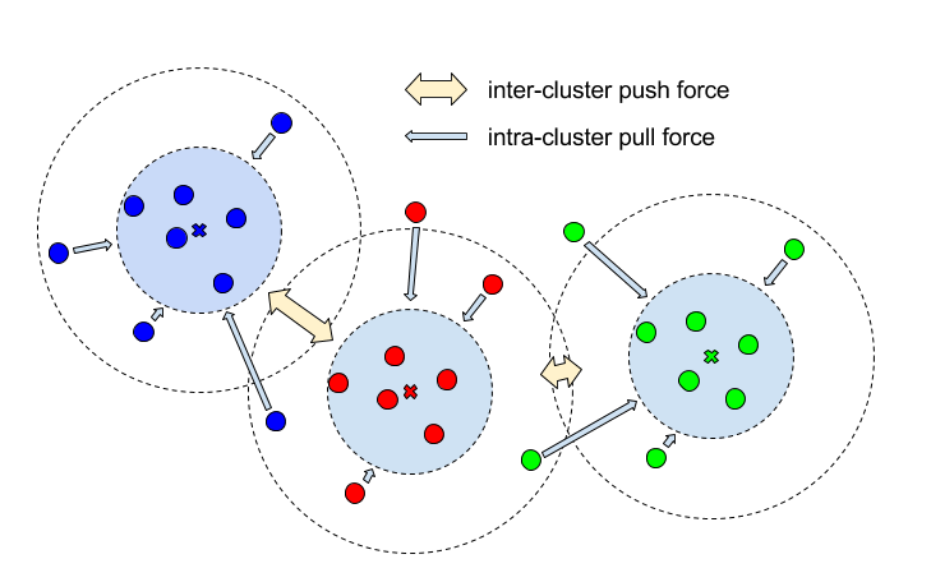
\includegraphics[width=0.5\textwidth]{figures/contrastive_loss.png}
	\caption{As defined by the loss, this are the hinged inter-pulling and intra-pushing forces acting on points in the embedding space \cite{brab2017semantic}}
	\label{fig_contrastive}
\end{figure}

\subsection{Triplet loss}\label{ssec:loss_triplet}
This loss, as defined in \cite{Schroff_2015} is related to the contrastive loss in section \ref{loss_contrastive} in the sense that it is also defined over data points in an embedding space where the resulting embeddings form ideally per instance clusters. The loss function expects three embedding vectors as an input. An anchor $x_i^a$, a embedding that is of the same class $x_i^p$ and one that is of a different class $x_i^n$. Then the loss yields

\begin{align}
	\mathcal{L}_{trpl} = \sum_i^N \left[ \norm{x_i^a - x_i^p}^2 - \norm{x_i^a - x_i^n}^2 + \alpha \right]_+ \text{\hspace{1mm}.}
\end{align} 

Again $[x]_+ = \max(0, x)$, $N$ is the number of all possible triplets $(x_i^a, x_i^p, x_i^n) \in \mathcal{T}$ in the embeddings, $\norm{\cdot}$ is the $L2$ norm and $\alpha$ is a enforced margin between positive and negative pairs. The training behavior using $\mathcal{L}_{trpl}$ as a loss is depicted in figure \ref{fig_triplet}. \\

\begin{figure}[ht!]
	\centering
	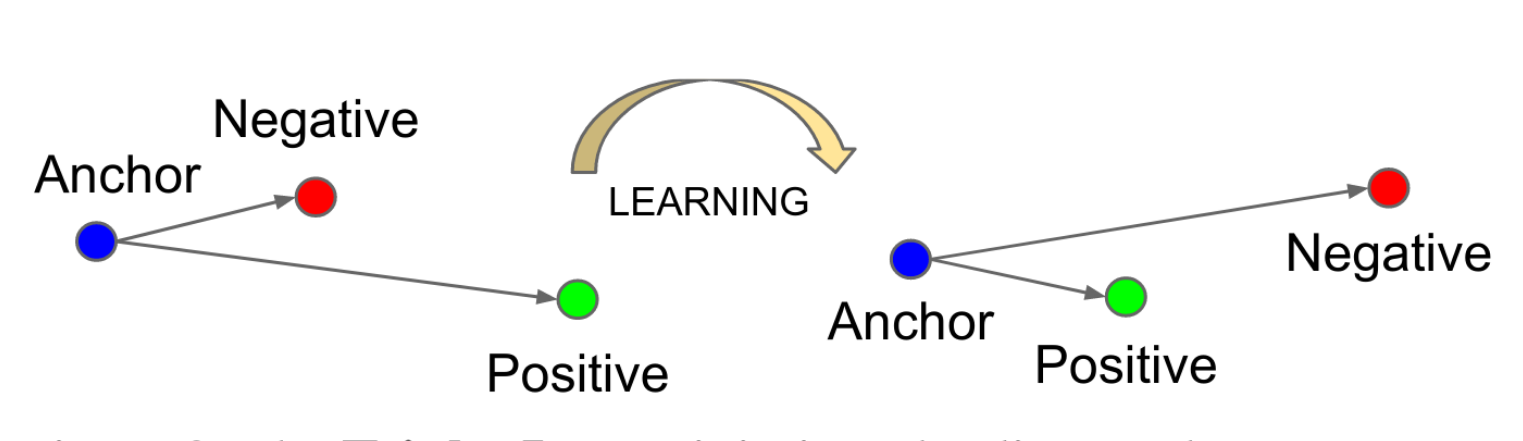
\includegraphics[width=0.5\textwidth]{figures/triplet_loss.png}
	\caption{Position of triplets in the embedding space before and after training \cite{Schroff_2015}}
	\label{fig_triplet}
\end{figure}

Often times $N$ is very large and the loss requires too many resources to calculate. Therefore it is crucial to select triples that are active, namely $\left\{ (x_i^a, x_i^p, x_i^n) \bigg| \left[ \norm{x_i^a - x_i^p}^2 - \norm{x_i^a - x_i^n}^2 + \alpha \right]_+ \neq 0 \right\}$ . However different selection strategies end in very different results regarding training time and convergence to satisfactory optima. E.g. picking only triplets that produce a high loss value can result in a training converging quickly into bad local optima.
To prevent the embeddings from diverging a regularizer term is added in order to constrain the embedding vectors to the unit hypersphere surface.
\begin{align}
	\mathcal{L}_{reg} = \sum_i^M\frac{1}{2}(\norm{x_i} - 1)^2
\end{align}

Here $M$ is the number of pixels in the image. The final loss therefore yields

\begin{align}
\mathcal{L} = \mathcal{L}_{trpl} + \beta \mathcal{L}_{reg}
\end{align}

where $\beta$ is a scalar weight for the regularizer term.
 \pagebreak



%\section*{References}
\setstretch{1.0}
\phantomsection~\label{sec:ref}
\addcontentsline{toc}{section}{References}
\bibliographystyle{IEEEtran}
\bibliography{bibliography.bib}
\pagebreak

\end{document}